\documentclass{beamer}
\usepackage{ctex}
\usepackage[export]{adjustbox}
\usepackage{listings}
\usepackage{xcolor}

\usetheme{focus}

\definecolor{codegreen}{RGB}{50 200 50}
\definecolor{codeblue}{RGB}{50 50 200}
\definecolor{codered}{RGB}{200 50 50}
\tikzset{
    global scale/.style={scale=#1,every node/.append style={scale=#1}},
    CC1/.style ={circle,minimum width = 30pt, minimum height =30pt, draw=black},
    CC2/.style ={circle,minimum width = 30pt, minimum height =30pt, draw=black, fill=blue!20},
    RA1/.style ={rectangle,minimum width = 30pt, minimum height =20pt, draw=black},
    RA2/.style ={rectangle,minimum width = 1cm, minimum height = 1cm, draw=black}
}

\title{算法分析与设计II}
\subtitle{2022-2023-2}
\date{Last Modified: 2023.1.16}
\institute{\vspace{2em} 数学与计算机学院 \\ 数据科学与大数据技术}
\titlegraphic{\vspace{5em} 
\includegraphics[scale=0.3]{fig/jlnu.pdf}}

\lstset{
    columns=flexible,       
    numbers=left,  
    numberstyle=\footnotesize\color{darkgray},  
    frame=shadowbox, 
    rulesepcolor= \color{gray}, 
    keywordstyle=\color{codeblue},         
    commentstyle=\color{codegreen},  
    stringstyle=\color{codered}, 
    showstringspaces=false,  
    xleftmargin=3em,
    xrightmargin=1em,              
    language=c++                           
}

\tikzset{
    CC1/.style ={
    circle,
    minimum width = 30pt, 
    minimum height =30pt, 
    draw=black
    }
}

\begin{document}
\frame{\titlepage}
\section{9. 计算几何}
\begin{frame}{9.1 点与线}
    \begin{itemize}
        \item 在计算几何中,采用\textcolor{blue}{向量}(vector,也称矢量)进行分析
        \item 空间中的点$p_1(x,y)$可以表示为向量$\vec{p_1}$,相当于原点指向该点的有向线段
        \item 两个向量的\textcolor{blue}{叉积}定义为:$\vec{p_1}\times \vec{p_2}=p_1.x\times p_2.y-p_2.x\times p_1.y$
        \item 空间两点$p_0,p_1$构成有向线段表示为向量$\vec{p_0p_1}$,$p_0,p_1$构成有向线段表示为向量$\overrightarrow{p_0p_1}$,以线段端点计算的叉积公式为:
        $$\begin{aligned}\overrightarrow{p_0p_1}\times \overrightarrow{p_0p_1}=(p_1.x-p_0.x)\times (p_2.y-p_0.y) \\\ -(p_2.x-p_0.x)\times (p_1.y-p_0.y) \end{aligned}$$
    \end{itemize}
\end{frame}
\begin{frame}{叉积的性质}
    \begin{itemize}
        \item $> 0$ 表明以$p_0$为公共点,线段$p_0p_1$在$p_0p_2$顺时针方向
        \item $< 0$ 表明以$p_0$为公共点,线段$p_0p_1$在$p_0p_2$逆时针方向
        \item $= 0$ 表明线段$p_0p_1$和$p_0p_2$共线
    \end{itemize}    
    \vfill
    经常用三个点的叉积值来判断点和线段的关系:
    \begin{itemize}
        \item $> 0$ 表明$p_2$在$p_0p_1$的逆时针方向
        \item $< 0$ 表明$p_2$在$p_0p_1$的顺时针方向
        \item $= 0$ 表明$p_2$在过$p_0p_1$的直线上
     \end{itemize}     
    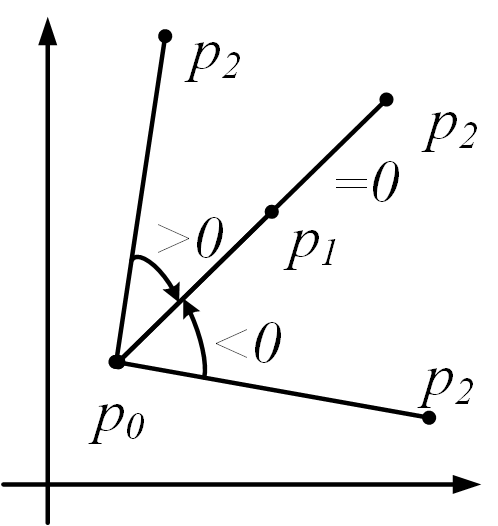
\includegraphics[width=0.3\textwidth,right]{fig/9-1.png}
\end{frame}
\begin{frame}{线段相交判断}
    \begin{itemize}
        \item $p_3p_4$和$p_3p_1$的叉积为负,$p_3p_4$与$p_3p_2$叉积为正,说明$p_1$和$p_2$跨立在$p_3p_4$两端,同理,$p_3$和$p_4$跨立在$p_1p_2$两端,两线段相交
        \item $p_3p_4$和$p_3p_1$的叉积为负, $p_3p_4$与$p_3p_2$叉积也为负,说明$p_1$和$p_2$在$p_3p_4$同侧,两线段不相交
    \end{itemize}  
    \vfill
    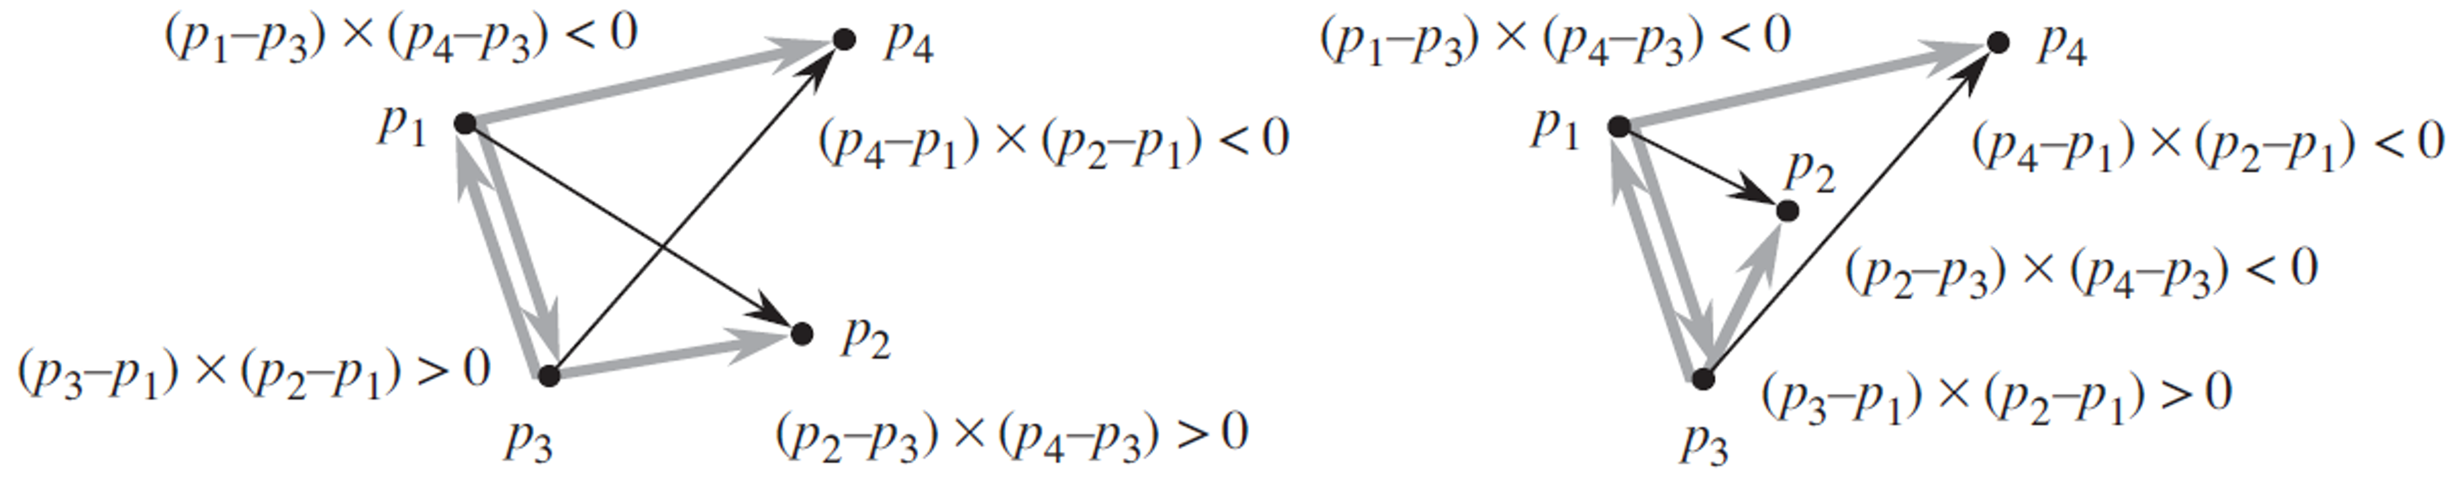
\includegraphics[width=0.9\textwidth,center]{fig/9-2.png}
\end{frame}
\begin{frame}{线段相交判断}

    \begin{center}
        \begin{tikzpicture}
        \filldraw (0,2) circle[radius=2pt] node[below]{$p_1$};
        \filldraw (1.5,1) circle[radius=2pt] node[above]{$p_3$};
        \filldraw (3,0) circle[radius=2pt] node[above]{$p_2$};
        \filldraw (3,2.4) circle[radius=2pt] node[above]{$p_4$};
        \filldraw (5,2) circle[radius=2pt] node[above]{$p_1$};
        \filldraw (8,0.5) circle[radius=2pt] node[above]{$p_2$};
        \filldraw (9,0) circle[radius=2pt] node[above]{$p_3$};
        \filldraw (8.2,2.4) circle[radius=2pt] node[above]{$p_4$};
        \draw[thick](0,2)--(3,0);
        \draw[thick](1.5,1)--(3,2.4);
        \draw[thick](5,2)--(8,0.5);
        \draw[thick](9,0)--(8.2,2.4);
        \node at(1.5,-1) {(a)};
        \node at(7,-1) {(b)};
    \end{tikzpicture}
    \end{center}
    \begin{itemize}
        \item 图(a),$p_3p_1$和$p_3p_2$的叉积为0,$p_3$在$p_1p_2$上,两线段相交
        \item 图(b), $p_3p_1$和$p_3p_2$的叉积为0, $p_3$在$p_1p_2$外,两线段不相交
    \end{itemize}  
    所以当叉积出现0时还需判断点是否在线段内,只要比较$p_3.x$是否在$p_1.x$和$p_2.x$之间,$p_3.y$是否在$p_1.y$和$p_2.y$之间,同时满足,则$p_3$在$p_1p_2$上
\end{frame}
\begin{frame}{1410 -- Intersection (poj.org)}
    \begin{itemize}
        \item You are to write a program that has to decide whether a given line segment intersects a given rectangle
        \item The line is said to intersect the rectangle if the line and the rectangle have at least one point in common. The rectangle consists of four straight lines and the area in between. Although all input values are integer numbers, valid intersection points do not have to lay on the integer grid.
    \end{itemize}  
    \begin{exampleblock}{An example:}
        \begin{columns}   
            \column{0.6\textwidth}
            \begin{itemize}
                \item line: start point: (4,9)
                \item end point: (11,2)
                \item rectangle: left-top: (1,5)
                \item right-bottom: (7,1)
            \end{itemize}
            \column{0.4\textwidth}
            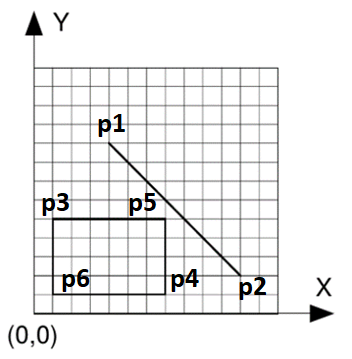
\includegraphics[width=0.7\textwidth]{fig/9-4.png}
        \end{columns}
    \end{exampleblock}
\end{frame}
\begin{frame}{9.2 多边形}
    \begin{columns}   
    \column{0.7\textwidth}
    \scriptsize{
    \begin{enumerate}[(1)]
        \item 叉积的另一种解释就是平行四边形的有向面积
        \item 有向三角形面积就可以通过叉积计算出来
        $$Area(p_0p_1p_2)=\frac{\overrightarrow{p_0p_1}\times \overrightarrow{p_0p_2}}{2}$$
        \item 以$p_1$为扇面中心,连接$p_1p_i$就得到$n-2$个三角形
        \begin{itemize}
            \item 由于凸性,保证这些三角形全在多边形内
            \item 由于叉积计算出来的面积是有正负的,所以面积也适用于凹多边形的情况
            $$A=\sum\limits_{i = 1}^{n-2}{A_i}$$
        \end{itemize}
        \item 将扇面中心移到(0,0)点,就可以得到更一般的面积公式
            $$A=\sum(x_iy_{i+1}+x_{i+1}y_i)$$
    \end{enumerate}}
    \column{0.3\textwidth}    
        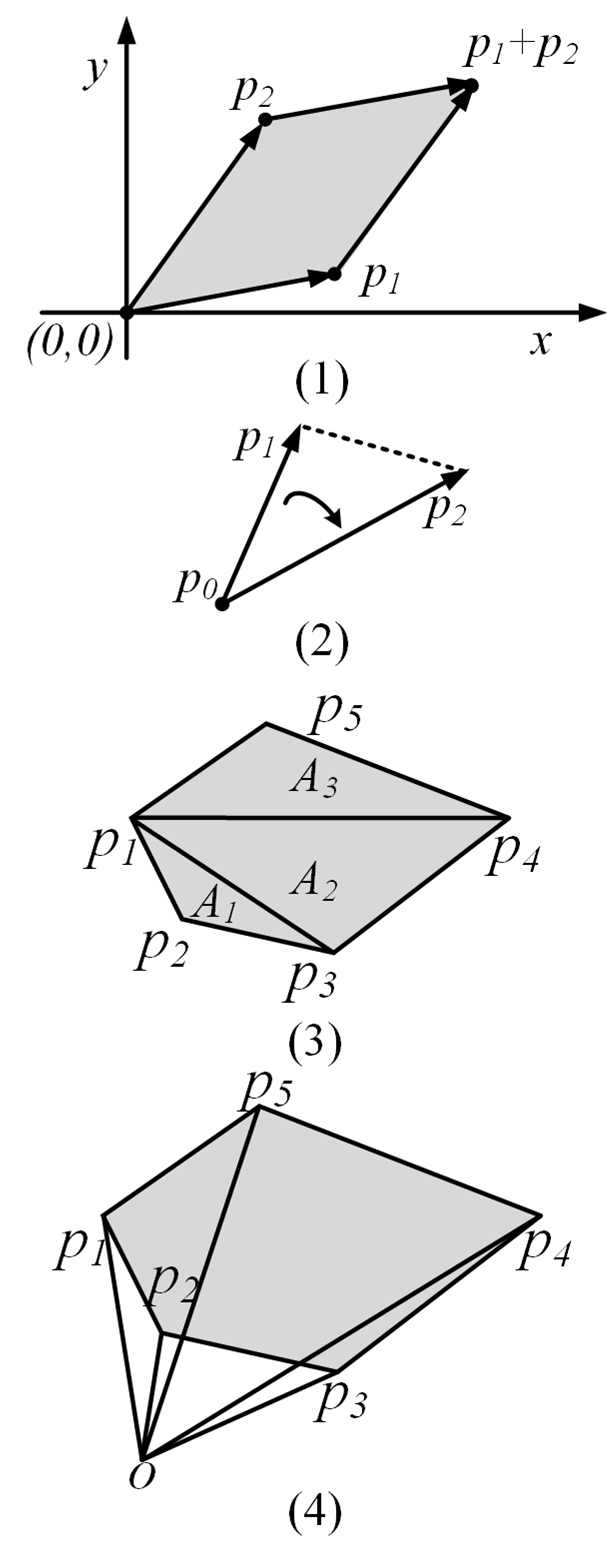
\includegraphics[width=0.8\textwidth]{fig/9-5.png}
    \end{columns}
\end{frame}
\begin{frame}{1269 -- Intersecting Lines (poj.org)}
    \begin{itemize}
        \item 给出4个点,判断通过前两点的直线和通过后两点直线的相互关系,相交、平行还是共线,相交的话求交点坐标
        \item 交点坐标用叉积(面积)属性来求,如图推导出交点$P$的公式为
        $$\frac{P_3P}{PP_4}=\frac{A_1}{A_2}=\frac{P_3-P}{P_4-P}\Rightarrow P=\frac{P_3\times A_2-P_4\times A_1}{A_2-A_1}$$
        其中:$A_1=Area(P_1P_2P_3),A_2=Area(P_1P_2P_4)$
        \item $A_1$和$A_2$都为0说明共线;$A_1$等于$A_2$说明平行;否则可以求出交点$P$
    \end{itemize} 
    \begin{center}
        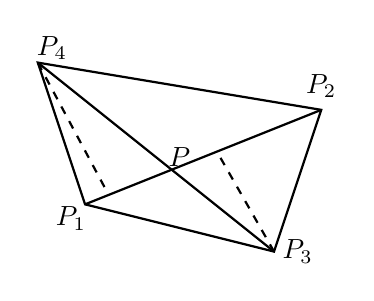
\begin{tikzpicture}[scale=0.6]
        \draw[thick] (1,1)--(0,4)--(6,3)--(5,0)--cycle;
        \draw[thick] (0,4)--(5,0);
        \draw[thick] (1,1)--(6,3);
        \draw[dashed,thick] (0,4)--(1.5,1.2);
        \draw[dashed,thick] (5,0)--(3.8,2.1);
        \node at(0.7,0.7) {$P_1$};
        \node at(0.3,4.3) {$P_4$};
        \node at(6,3.5) {$P_2$};
        \node at(5.5,0) {$P_3$};
        \node at(3,2) {$P$};
    \end{tikzpicture} 
    \end{center}
    
\end{frame}
\begin{frame}{3348 -- Cows (poj.org)}
    \begin{itemize}
        \item 给出$n$棵树的坐标$p(x,y)$,用这些树围成牧场,每头牛至少需要50平方米活动区间,问牧场最多能放下多少头牛
    \end{itemize} 
    \vfill
    \begin{block}{凸包}
        凸包(Convex hull) 的问题,即找一个包含所有点的最小凸多边形,所有的点要么在多边形的边上,要么在其内部
    \end{block}
\end{frame}
\begin{frame}{葛立恒扫描法(Graham's scan)}
    \begin{itemize}
        \item 在所有点中选择左下点作为$p_0$,将剩余点按照\textcolor{blue}{极角}大小排序,之后将$p_0,p_1$放入栈中,计算次栈顶点、栈顶点和下一个顺序点的叉积值,如果为正,栈顶保留,如果为负,则栈顶点出栈;下一个顺序点入栈,继续以上操作,最后栈中的点就是所求凸包的顶点
    \end{itemize}
    \begin{exampleblock}{例}
        多边形$p_2p_7p_8p_5p_9$为点集$\{ p_1,p_2,\ldots ,p_9\}$的凸包
        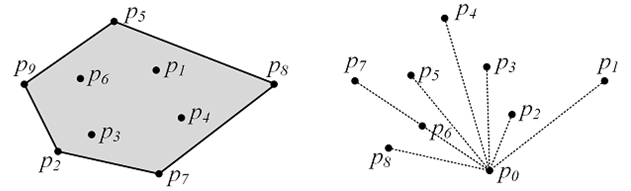
\includegraphics[width=0.8\textwidth,center]{fig/9-7.png}
    \end{exampleblock}
\end{frame}
\end{document}